\documentclass [titlepage,12pt,letter] {article}
\pagestyle{myheadings}


\usepackage{graphicx} 
\usepackage{epsfig}
\usepackage{subfigure}
\usepackage{fancyhdr}
\usepackage{url} 
\usepackage{amsmath}
\usepackage{algorithm} 
\usepackage{algorithmic}
\pagestyle{fancy}



\fancyhead{}
\fancyfoot{}
			
\lhead{CSC349A Lecture Notes}
\rhead{Little, Rich}


\setcounter{page}{1}
\cfoot{\thepage}




\begin{document} 


These are the lecture notes for CSC349A Numerical Analysis taught by
Rich Little. They roughly correspond to
the material covered in each lecture in the classroom but the actual
classroom presentation might deviate significantly from them depending
on the flow of the course delivery. They are provided as a reference to
the instructor as well as supporting material for students who miss
the lectures. They are simply notes to support the lecture so the text
is not detailed and they are not thoroughly checked. Use at your own
risk. They are complimentary to the handouts. Many thanks to all the
guidance and materials I received from Dale Olesky who has taught this
course for many years and George Tzanetakis. 

\section{Higher-Order Taylor Series Methods}

Higher order methods can be obtained by keeping more terms from the Taylor expansion.
\begin{multline*}
y(x_{i+1})=y(x_i)+hy'(x_i)+\frac{h^2}{2}y''(x_i)+\dotsm \\
	+\frac{h^n}{n!}y^{(n)}(x_i)+\frac{h^{n+1}}{(n+1)!}y^{(n+1)}(\xi_i) \\
=y(x_i)+hf(x_i,y(x_i))+\frac{h^2}{2}f'(x_i,y(x_i))+\dotsm \\
	+\frac{h^n}{n!}f^{(n-1)}(x_i,y(x_i))+O(h^{n+1})
\end{multline*}

\subsection{The Taylor Method of Order $n$}

Dropping the $O(h^{n+1})$ remainder term in the above Taylor expansion, gives a numerical method
\begin{multline*}
y_{i+1}=y_i+hf(x_i,y_i)+\frac{h^2}{2}f'(x_i,y_i)+\dotsm 
	+\frac{h^n}{n!}f^{(n-1)}(x_i,y_i)
\end{multline*}
for any integer $n \geq 1$.

This is called {\bf the Taylor method of order $n$} (as its local truncation error is $O(h^{n+1})$, and thus its global truncation error is $O(h^n)$).

Euler’s method is just the case when $n=1$.


\subsubsection{Example 1: Taylor Method of Order 2}

Solve the differential equation $y'=y-x^2+1$ with $y(0)=0.5$ using the Taylor Method of order $n=2$ with step size $h=0.2$.

\vspace{\baselineskip}

The Taylor Method of order 2 is
\[
y_{i+1}=y_i + hf(x_i,y_i) + \frac{h^2}{2}f'(x_i,y_i)
\]
where
\[
f'(x,y(x)) = (y-x^2+1)' = y' - 2x = y-x^2+1-2x
\]
So,
\begin{align*}
y_{i+1} &= y_i + h(y_i - x_i^2 +1) + \frac{h^2}{2}(y_i - x_i^2 +1 - 2x_i) \\
&= y_i + h \left [((y_i - x_i^2 +1) + \frac{h}{2}(y_i - x_i^2 +1) - hx_i \right ] \\
&= y_i + h \left [(1+\frac{h}{2})(y_i - x_i^2 +1)  - hx_i \right ]
\end{align*}

Thus, at $(0,0.5)$ with $h=0.2$ we get
\begin{align*}
y_1 &= y_0 +  h \left [(1+\frac{h}{2})(y_0 - x_0^2 +1)  - hx_0 \right ] \\
&= 0.5 +(0.2)\left [(1 + 0.1)(0.5 - 0^2 +1) - (0.2)(0) \right ] \\
&= 0.5 + (0.2)(1.1)(1.5) \\
&= 0.83
\end{align*}

Recall from last lecture, the true value is $y(0.2)=0.8292986$ and Euler's method gave $y_1=0.8$, so the order 2 method gained another significant digit.

{\bf Problems with higher-order Taylor Methods:}
For $n \geq 2$, use of a Taylor method requires evaluation of the derivatives of the function $f(x,y(x))$ with respect to $x$. Although the Taylor methods of order $n$ have high accuracy for values of $n = 3, 4 \text{ or } 5$, they are seldom used in practice because of the difficulty and expense in evaluating the required higher derivatives. Runge-Kutta methods are a class of higher-order methods that are more often used in practice.

\section{Runge-Kutta Methods}

Advantage of Taylor methods of order $n$
\begin{itemize}
\item{global truncation error of $O(h^n)$ insures high accuracy (even for $n = 3, 4$ or $5$)}
\end{itemize}
Disadvantage
\begin{itemize}
\item{high order derivatives of $f(x,y(x))$ may be difficult and expensive to evaluate.}
\end{itemize}
\vspace{\baselineskip}
{\bf Runge-Kutta methods} are higher order formulas (they can have any order $\geq 1$) that require function evaluations only of  $f(x,y(x))$, and not of any of its derivatives. Runge-Kutta methods are so-called one-step methods (as also are Euler’s method and all Taylor methods): that is, they are of the form
\[
y_{i+1}=y_i+h\Phi(x_i,y_i,h)
\]
for some (possibly very complicated) function $\Phi$.  

That is, each computed approximation $y_{i+1}$ is computed using only the value $y_i$ at the previous grid point, along with the values of $x_i$, the step size $h$, and of course the function $f(x,y(x))$ that specifies the differential equation.

A fundamental source of error in Euler's method is that the derivative at the beginning of the interval is assumed to apply across the entire interval. There are ways to circumvent this shortcoming and inprove our method without adding more Taylor terms. I will illustrate two such Runge-Kutta methods, both of which are order 2 methods (as opposed to Euler's method which is an order 1 meethod.)

\subsection{General Form of RK Methods of Order $m$} 

A Runge-Kutta method of order $m$ is of the form:
\[
y_{i+1}=y_i+h\sum_{j=1}^m a_jk_j
\]
where the $a_j$ are constants and the $k_j$ are functions of the form,
\begin{align*}
k_1&=hf(x_i,y_i) \\
k_j&=hf(x_i+\alpha_jh,y_i+h\sum_{l=1}^{j-1}\beta_{jl}k_l), \text{ for } 2 \leq j \leq m
\end{align*}

{\bf Examples:} Derive the general forms for $m=1,2,3,$ and $4$.

Each of these formuals defines a whole class of Runge-Kutta methods of order $m$.

Our goal is to take the formula for any fixed value of $m \geq 1$, and determine values for the parameters:
\begin{itemize}
\item{$\{a_1 \}$ when $m=1$}
\item{$\{a_1,a_2,\alpha_2,\beta_{21} \}$ when $m=2$}
\item{$\{a_1,a_2,a_3,\alpha_2,\alpha_3,\beta_{21},\beta_{31},\beta_{32} \}$ when $m=3$}
\item{$\{a_1,a_2,a_3,a_4,\alpha_2,\alpha_3,\alpha_4,\beta_{21},\beta_{31},\beta_{32},\beta_{41},\beta_{42},\beta_{43} \}$ when $m=4$}
\end{itemize}
so that the resulting Runge-Kutta method has as high an order as possible (i.e., its local truncation error is as small as possible).

\section{Derivation of Runge-Kutta Methods}

This is accomplished by choosing the unknown parameters $\{a_i\},\{\alpha_i\}$, and $\{\beta_{ij}\}$ so that the Runge-Kutta formula
\[
y_{i+1}=y_i+h\sum_{j=1}^m a_jk_j
\]
is identical to the Taylor series expansion
\[
y(x_{i+1})=y(x_i)+hy'(x_i)+\frac{h^2}{2}y''(x_i)+\frac{h^3}{6}y'''(x_i)+\dotsm
\]
to as many terms as possible.

{\bf Case  m = 1}
 
The only Runge-Kutta method of first order is when $a_1=1$. That is, Euler’s method
\[
y_{i+1}=y_i+hf(x_i,y_i)
\]
For each value of $m \geq 2$, there are an infinite number of Runge-Kutta formulas, each one having local truncation error $O(h^{m+1})$ and thus global truncation error $O(h^m)$.

\subsection{Taylor Polynomial with 2 Variables} 

This is accomplished using the Taylor polynomial for a function of 2 variables:
\begin{multline*}
f(x+h,y+k)=f(x,y)+hf_x(x,y)+kf_y(x,y) \\
	+\frac{h^2}{2}f_{xx}(x,y) + hkf_{xy}(x,y)+\frac{k^2}{2}f_{yy}(x,y) \\
	+\frac{h^3}{6}f_{xxx}(x,y)+\frac{h^2k}{2}f_{xxy}(x,y)+\frac{hk^2}{2}f_{xyy}(x,y)+\frac{k^3}{6}f_{yyy}(x,y) \\
	+ \dotsm
\end{multline*}
where $f_x \equiv \frac{\partial f}{\partial x}, f_{xy} \equiv \frac{\partial^2 f}{\partial x \partial y}$, etc.

The derivation of Runge-Kutta methods and an understanding of why they work requires the Taylor polynomial for a function of 2 variables, but this Taylor polynomial is not required to use these methods to numerically approximate the solution of a differential equation.

\subsection{Derivation of second order R-K} 

\begin{align*} 
y(x_{i+1}) &=  y(x_i) + a_1 h f(x_i, y_i)  \\
   &+ a_2 h f(x_i + \alpha_2 h, y_i + \beta_{21}hf(x_i,y_i))  \\ 
\end{align*} 
Using the Taylor exapnsion for $f(x_i + \alpha_2 h, y_i + \beta_{21}hf(x_i,y_i))$, we get
\begin{multline*} 
y(x_{i+1}) = y(x_i) + a_1 h f(x_i, y_i)+ a_2 h [ f(x_i,y_i) +   \alpha_2hf_x(x_i,y_i) \\
+ \beta_{21} h f (x_i, y_i) f_y(x_i,y_i) + O(h^2) ] \\
= y(x_i) + [a_1 + a_2] h f(x_i, y_i) + h^2 [ a_2 \alpha_2 f_x(x_i,y_i) \\
+ a_2 \beta_{21}f(x_i,y_i)f_y(x_i,y_i)] + O(h^3) 
\end{multline*} 

But, also by Taylors Theorem 
\begin{align*} 
y(x_{i+1}) =& y(x_i) + h y'(x_i) + \frac{h^2}{2} y''(x_i) + O(h^3) \\
	=& y(x_i) + hf(x_i,y_i) + \frac{h^2}{2} f'(x_i,y_i) + O(h^3) \\
           =& y(x_i) + h f(x_i, y_i) + \frac{h^2}{2}[f_x(x_i,y_i) + f(x_i,y_i) f_y(x_i,y_i)] \\ 
	+& O(h^3) 
\end{align*} 
These two are equal only when \[a_1+a_2=1, a_2 \alpha_2=1/2,a_2 \beta_{21}=1/2\]


\subsection{Heun's Method} 

The first method uses Euler's method to estimate the slope at $x_{i+1}$ and then average that with the slope at $x_i$, giving a better estimate of the average slope over the subinterval from $x_i$ to $x_{i+1}$. 

Recall that in Euler's method, the slope at $x_i$ is given by
\[
y_i'=f(x_i,y_i)
\]
which is used to approximate $y(x_{i+1})$ by
\[
y^E_{i+1}=y_i+f(x_i,y_i)h
\]
where $y^E_{i+1}$ denotes the Euler approximation of $y(x_{i+1})$. The textbook calls this the {\it predictor equation}.

We can now use $y^E_{i+1}$  to approximate the slope at $y(x_{i+1})$ by
\[
y'_{i+1}=f(x_{i+1},y^E_{i+1})
\]

Putting these two together gives us Heun's method,
\[
y_{i+1}=y_i+\frac{h}{2}\left[f(x_i,y_i)+f(x_i+h,y_i+hf(x_i,y_i))\right]
\]

\begin{figure}[h] 
  \centering
  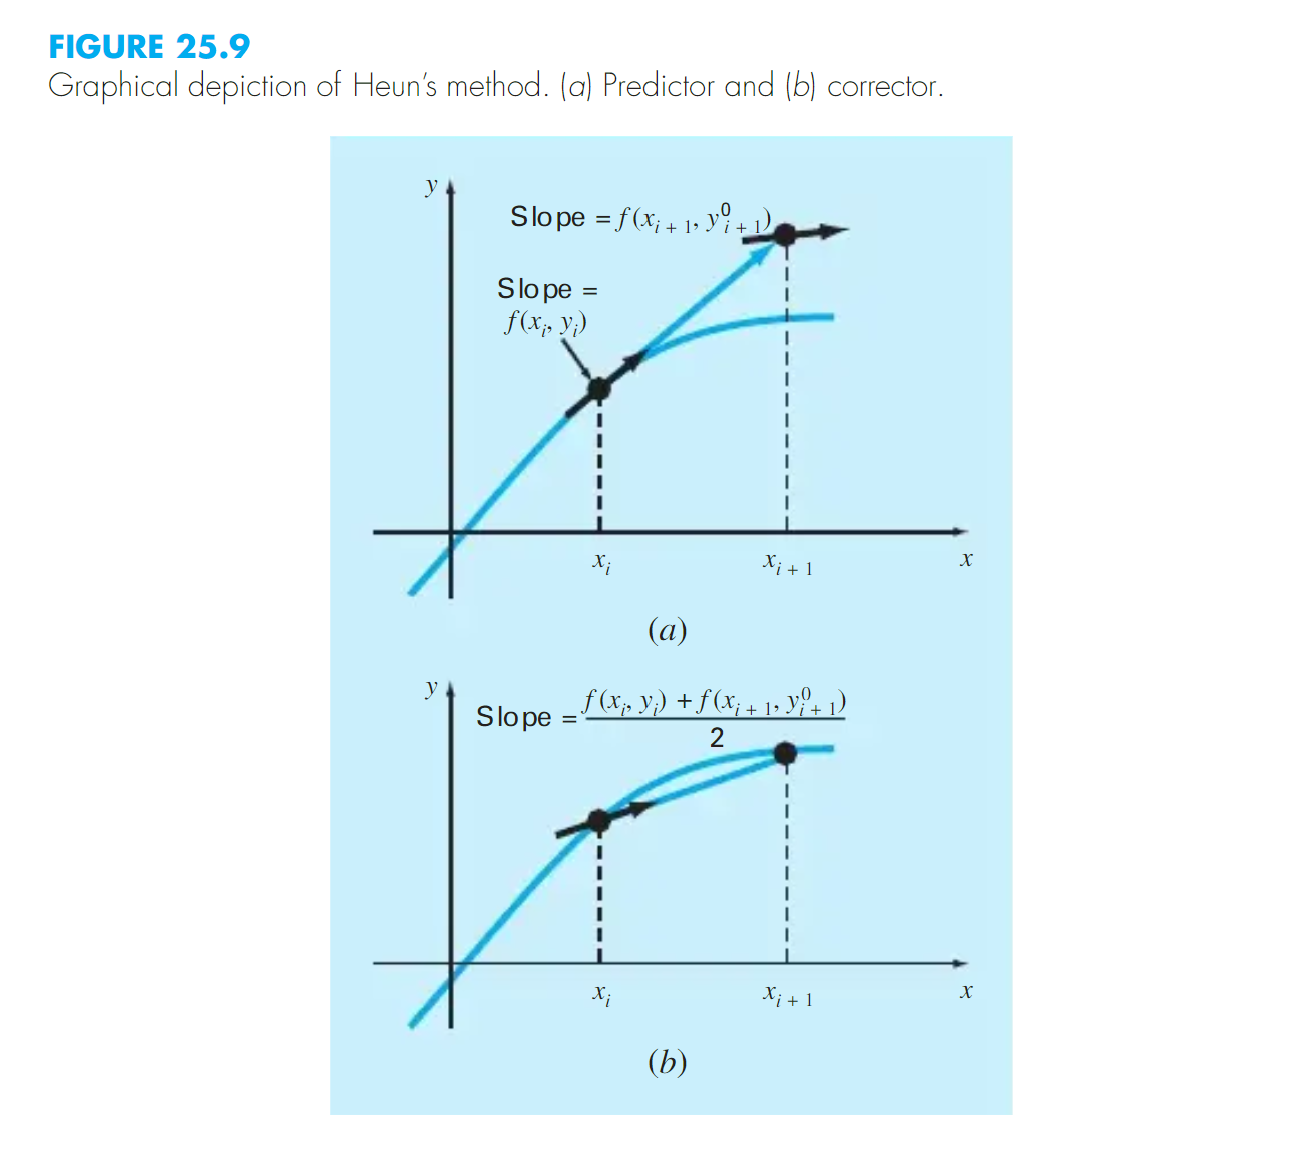
\includegraphics[scale=0.8]{figure25-9}
  \label{fig:Heun}
\end{figure}


\subsubsection{Example 2}Use Heun's Method to solve $y'=4e^{0.8x}-0.5y$ from $x=0$ to $x=4$ with $h=1$ and $y_0=2$. According to Heun's method,
\begin{align*}
y_1&=y_0+\frac{h}{2}\left[f(x_0,y_0)+f(x_0+h,y_o+hf(x_0,y_0))\right] \\
&=2+\frac{1}{2}\left[f(0,2)+f(0+1,2+f(0,2))\right]
\end{align*}
where
\[
f(0,2)=4e^{0.8(0)}-0.5(2)=4-1=3
\]
So,
\begin{align*}
y_1&=2+\frac{1}{2}\left[3+f(1,5)\right]
\end{align*}
where
\[
f(1,5)=4e^{0.8(1)}-0.5(5)=6.402164
\]
Thus,
\begin{align*}
y_1&=2+\frac{1}{2}\left[3+6.402164\right] \\
&=6.701082
\end{align*}

Note that the true value is $y(1)=6.1946314$, giving a relative error of
\[
|\varepsilon_t|=\left|\frac{6.1946314-6.701082}{6.1946314}\right|\approx 8\%
\]

We can use Heun's method in an interative manner to get a better approximation at $x_1$ before we move on to $x_2$, by making are first approximation above the predictor and applying Heun's method at $x_0$ again, so
\begin{align*}
y_1&=2+\frac{1}{2}\left[3+f(1,6.701082)\right] \\
&=2+\frac{1}{2}\left[3+4e^{0.8(1)}-0.5(6.701082)\right] \\
&=6.275811
\end{align*}

The relative error for this approximation is
\[
|\varepsilon_t|=\left|\frac{6.1946314-6.275811}{6.1946314}\right|\approx 1.31\%
\]

We can continue on in this manner until we find the error acceptable.

\subsection{Midpoint Method:} The other second order Runge-Kutta method uses the slope approximation at the midpoint of the subinterval, at point $x_{i+1/2}=x_i+h/2$, to find $y_{i+1}$, giving equation
\[
y_{i+1}=y_i+hf\left(x_i+\frac{h}{2},y_i+\frac{h}{2}f(x_i,y_i)\right)
\]

\begin{figure}[h] 
  \centering
  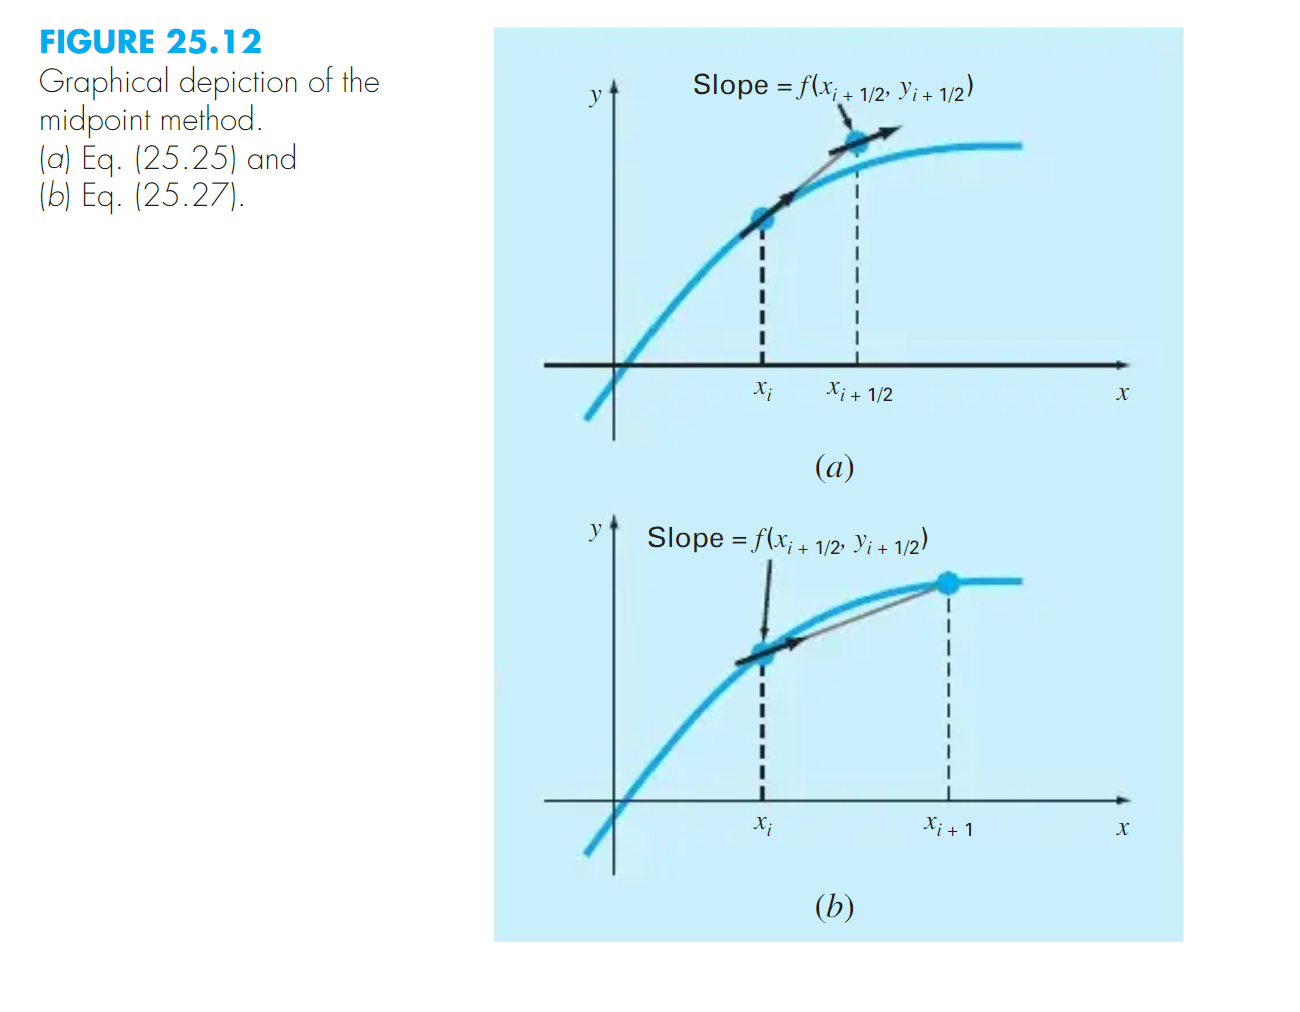
\includegraphics[scale=0.8]{figure25-12}
  \label{fig:Midpoint}
\end{figure}

\subsubsection{Example 2}Use the Midpoint Method to solve $y'=4e^{0.8x}-0.5y$ from $x=0$ to $x=4$ with $h=1$ and $y_0=2$. According to the Midpoint method,
\begin{align*}
y_1&=y_0+hf\left(x_0+\frac{h}{2},y_0+\frac{h}{2}f(x_0,y_0)\right) \\
&=2+(1)f\left(0+\frac{1}{2},2+\frac{1}{2}f(0,2)\right) \\
&=2+f\left(0.5,2+\frac{1}{2}(3)\right) \\
&=2+f\left(0.5,3.5\right)
\end{align*}
where
\[
f(0.5,3.5)=4e^{0.8(0.5)}-0.5(3.5)=4.21729879
\]
Thus,
\begin{align*}
y_1&=2+4.21729879 \\
&=6.21729879
\end{align*}

Note that the true value is $y(1)=6.1946314$, giving a relative error of
\[
|\varepsilon_t|=\left|\frac{6.1946314-6.21729879}{6.1946314}\right|\approx 0.37\%
\]

\subsection{Derivation of Third Order RK Methods}  

{\bf Case  m = 3}
It can be shown that any solution of a certain system of 6 nonlinear equations in 8 unknowns gives a third-order Runge-Kutta Method.

One common solution is
\[
a_1=\frac{1}{6}, a_2=\frac{2}{3}, a_3=\frac{1}{6}, \alpha_2=\frac{1}{2}, \alpha_3=1, \beta_{21}=\frac{1}{2}, \beta_{31}=-1, \beta_{32}=2
\]
which gives the third-order Runge-Kutta method
\[
y_{i+1}=y_i+\frac{h}{6}(k_1+4k_2+k_3)
\]
where
\begin{align*}
k_1 &= f(x_i,y_i) \\
k_2 & = f\left(x_i+\frac{h}{2},y_i+\frac{h}{2}k_1\right) \\
k_3 &= f(x_i+h,y_i-hk_1+2hk_2)
\end{align*}

\subsection{Derivation of Fourth Order RK Methods}  

{\bf Case  m = 4}
The 13 Runge-Kutta parameters are obtained by solving 11 nonlinear equations in 13 unknowns. One solution is called the {\bf "classical" Runge-Kutta method}, which has global truncation error of $O(h^4)$:

\[
y_{i+1}=y_i+\frac{h}{6}(k_1+2k_2+2k_3+k_4)
\]
where
\begin{align*}
k_1 &= f(x_i,y_i) \\
k_2 & = f\left(x_i+\frac{h}{2},y_i+\frac{h}{2}k_1\right) \\
k_3 & = f\left(x_i+\frac{h}{2},y_i+\frac{h}{2}k_2\right) \\
k_4 &= f(x_i+h,y_i+hk_3)
\end{align*}

\end{document} 















